%%% Local Variables:
%%% TeX-command-extra-options: "--shell-escape"
%%% End:

\documentclass[aspectratio=169]{beamer}
\usepackage[pdf]{graphviz}
\usetheme{Bruno}

\usepackage{mathtools}
\usepackage{asymptote}
\title{Shannon's Noisy Channel Theorem over a Binary Symmetric Channel}
\author{
    Ramesh Balaji
}
\institute{Rutgers University}
\date{\today}
\newcommand{\re}{\color{red}}
\newcommand{\gr}{\color{green}}
\newcommand{\bl}{\color{blue}}
\newcommand{\bigfloor}[1]{\Bigl \lfloor #1 \Bigr \rfloor}
\newcommand{\floor}[1]{\lfloor #1 \rfloor}
\newcommand{\ceil}[1]{\lceil #1 \rceil}
\newcommand{\bigceil}[1]{\Bigl \lceil #1 \Bigr \rceil}

\begin{document}

\maketitle

\begin{frame}{Context}
\begin{itemize}
  \item Data transfer is unreliable
  \item Eg. sending data over a network, eg. using TCP or UDP
  \item Have to find a way to correct data
  \item \textbf{Error-correcting codes (ECCs): }method to correct data after transmission
\end{itemize}
\end{frame}



\begin{frame}{Context: Representing Data}
\begin{itemize}
    \item Data transmitted can be represented as an array of bits.
    \item Array of bits as a column vector of $3$ bits: \(\begin{bmatrix} 0 \\ 1 \\ 1 \end{bmatrix}.\)
    \item The set of all bitstrings with $3$ bits is denoted as $\{0, 1\}^{3}$. Similarly, for $n$ bits, this is given as $\{0, 1\}^{n}$.
\end{itemize}
\end{frame}


\begin{frame}{Context: Encoder and Decoder Function}
\begin{itemize}
  \item ECCs have a \textbf{encoder} and \textbf{decoder}
  \item Encoder adds \textit{additional data} to original data.
        \begin{itemize}
            \item This extra data is used after transmission to recover the original data
            \item Given as a function $f: \{0, 1\}^{n} \to \{0, 1\}^{m}$.
            \item Since there are more bits in the result, $m > n$.
          \end{itemize}
    \item Decoder converts the \textit{transmitted data} to the original message.
        \begin{itemize}
            \item Given as a function $g: \{0, 1\}^{m} \to \{0, 1\}^{n}$.
          \end{itemize}
    \item \textit{Noise} from transmitting $f(\vec{x})$ over the channel.
        \begin{itemize}
              \item Given as a vector $E \in \{0, 1\}^{m}$
              \item Mathematically, added to the result $f(\vec{x})$ where addition is mod 2 (example will be provided later).
          \end{itemize}
\end{itemize}
\end{frame}

\begin{frame}{Context: Encoder and Decoder}
\digraph[scale=0.7]{encodingscheme}{
    rankdir=LR;
    node [shape=rectangle];
    x_orig [shape=circle, style=filled, label = "x"];
    x_out [shape=circle, style=filled, label = "x"];
    Noise [style=filled, fillcolor=coral];
    f [style=filled, fillcolor=cyan3, label="f\noexpand\nEncoder"];
    g [style=filled, fillcolor=cyan3,  label="g\noexpand\nDecoder"];
    x_orig -> f;
    f -> Noise [label = "f(x)"];
    Noise -> g  [label = "f(x) + E"];
    g -> x_out [label = "g(f(x) + E)"];
}

\end{frame}

\begin{frame}{Context: Binary Symmetric Channel}
  \begin{itemize}
      \item How is the error vector $E \in \{0, 1\}^{n}$ generated?
      \item Different kinds of channels generate different types of noise.
      \item \textbf{Binary Symmetric Channel (BSC):} the probability of a bit flip in the input is $p$.
          \begin{itemize}
                  \item More mathematically, if $E_{i}$ represents the $i$th bit in $E$, then \( E_{i} = \begin{cases} 1 & \text{w.p. $p$} \\ 0 & \text{w.p $1-p$}\end{cases}\)
                  \item Then, when $E$ is added to the input vector $f(\vec{x})$, it represents the output data \textit{after} transmission over the channel.
            \end{itemize}
    \end{itemize}
\end{frame}


\begin{frame}{Example: Basic Error-Correction Code over a BSC}
\begin{itemize}
  \item \textbf{Encoder} will repeat every bit $3$ times. Of every block, \textbf{decoder} will choose the bit in the block that occurs the most.
  \begin{itemize}
          \item $f: \{0, 1\}^{n} \to \{0, 1\}^{3n}$
          \item $g: \{0, 1\}^{3n} \to \{0, 1\}^{n}$
    \end{itemize}
  \item Our message is \(\vec{x} = \begin{bmatrix} \re1 \end{bmatrix}\). Using row vectors to save space.
  \item \(f(\vec{x}) = \begin{bmatrix} \re1 & \re1 & \re1 \end{bmatrix}\)
  % Could autogenerate/make interactive??
  \item Suppose $p = 0.1$ and \(E = \begin{bmatrix} 0 & 1 & 0\end{bmatrix}\). \\ \begin{tabular}{ccccc}
            & f(x)     & \re1 & \re1 & \re1\\
          + & E        & 0 & 1 & 0\\
          \hline
            & f(x) + E & \re1 & \re0 & \re1
          \end{tabular}

\end{itemize}
\end{frame}

\begin{frame}{Example: Basic Error-Correction Code over a BSC (Cont.)}
  \begin{itemize}
  \item Decoding: \( f(\vec{x}) + E =\begin{bmatrix}\re1 & \re0 & \re1 \end{bmatrix}\)
          \begin{itemize}
                \item Most common bit is \textbf{1}, so the output is \(\begin{bmatrix} 1 \end{bmatrix}\).
                  \end{itemize}
    \item Output \(g(f(\vec{x}) + E) = \begin{bmatrix}\re1\end{bmatrix} = \vec{x}\).
          \begin{itemize}
                  \item Despite errors in the transmission, we still could decode the original message.
                  \end{itemize}
          \end{itemize}
  \end{frame}


\begin{frame}{Statistics on Example Transmission Scheme}
  \begin{itemize}
    \item The encoder function is defined as $f: \{0, 1\}^{m} \to \{0, 1\}^{n}$
    \item The \textbf{rate of transmission} is defined as $\frac{m}{n}$.
          \begin{itemize}
            \item For the example code, the rate of transmission $R = \frac{1}{3}$.
            \end{itemize}
    \item \textbf{Probability of failure} of our sample code:
          \begin{itemize}
                \item We need to find the probability that either $E$ has two $1$s or three $1$s.
                \item $\binom{3}{2} p^{2}(1-p) + \binom{3}{3} p^{3} = 0.028 $
            \end{itemize}
          \end{itemize}
  \end{frame}
\begin{frame}{Tradeoff Between Rate of Transmission and Probability of Failure}
  \begin{itemize}
    \item What if we copy the bit more times?
          \begin{itemize}
                \item If repeated $n$ times, then $R = \frac{1}{n}$
                \item Probability of failure? Must be at least $\ceil{\frac{n}{2}}$ $1$s in $E$ for failure.
            \item $P[g(f(x) + E) \ne x] = \sum_{i=\ceil{\frac{n}{2}}}^n \binom{n}{i}p^{i}(1-p)^{n-i} $
            \item Probability of failure for $n$ repeated bits\\ \begin{minipage}{\linewidth}  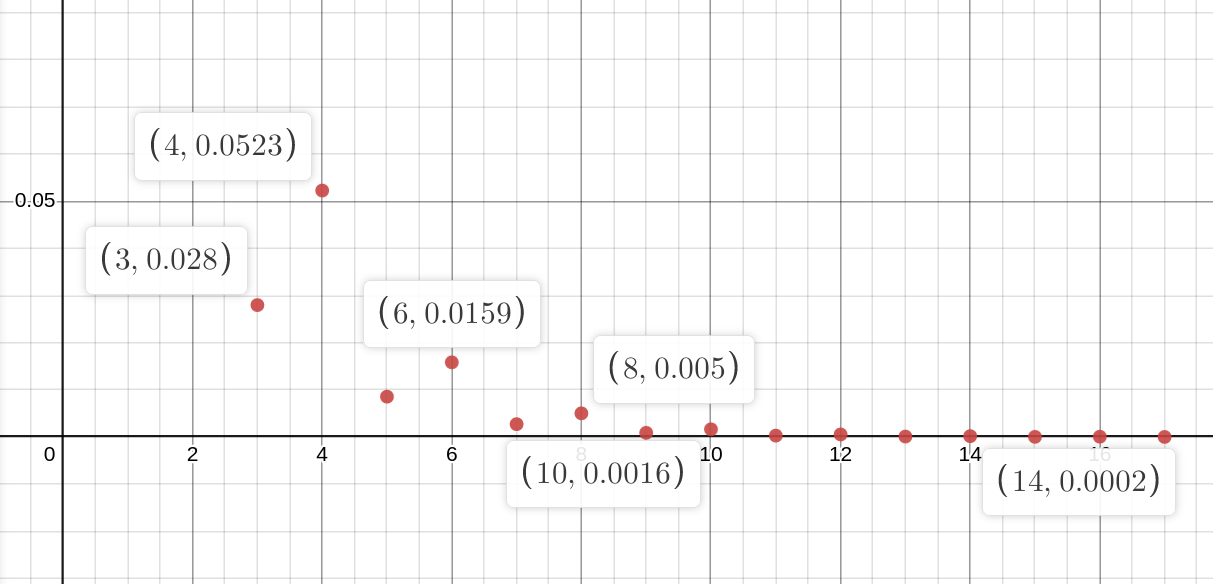
\includegraphics[width=0.5\textwidth]{repeated_bit_prob} \end{minipage}
            \item Observation: worse rate of transmission ($\frac{1}{n}$), but lower probability of failure.
          \end{itemize}
    \end{itemize}
  \end{frame}

  \begin{frame}{Shannon's Noisy Channel Coding Theorem over BSC}
      \begin{itemize}
        \item Shannon's Noisy Channel Coding Theorem proves the existence ECC scheme with \textit{theoretical} rate of transmission and failure probability.
        \item For a BSC with bit-flip probabliity $p$, for some arbitrarily small $\epsilon > 0$, there exists some ECC scheme with rate of transmission $1 - H(p) - \epsilon$, and probability of failure less than $\epsilon$.
              \begin{itemize}
                      \item Note that $H(p) = -p\log_{2}{p}-(1-p)\log_{2}{1-p}$, which is the binary entropy function.
                \end{itemize}
        \item Does not tell us \textit{what} that ECC scheme is, but states there exists one.
        \end{itemize}
    \end{frame}

    \begin{frame}{``Proving'' the Noisy Channel Coding Theorem}
      \begin{itemize}
      \item Not a formal proof.
      \item \textbf{Two steps:}
        \begin{enumerate}
                \item Define a coding scheme with the appropriate rate of transmission
                \item Prove that its probability of failure is less than $\epsilon$.
                \end{enumerate}
              \end{itemize}
      \end{frame}

    \begin{frame}{Defining an ECC}
          \begin{itemize}
                \item Define $\delta$ such that $p + \delta < 0.5$, and $H(p + \epsilon)< H(p) + \delta$.
                \item \textbf{Encoder:} $f: \{0, 1\}^{n(1-H(p)-\epsilon)} \to \{0, 1\}^{n}$. Thus the rate of transmission is correct.
                  \begin{itemize}
                \item Given an input, $f$ will output a random vector in $\{0, 1\}^{n}$ (there are some problems with this, namely that $f$ could end up not being a function, but I think the probability is low)
                          \end{itemize}
                \item \textbf{Decoder:} $g: \{0, 1\}^{n} \to \{0, 1\}^{n(1-H(p)-\epsilon)}$.
                  \begin{itemize}
                      \item Given transmitted data $f(\vec{x}) + E$, choose the value $\vec{y} \in f(\{0, 1\}^{n})$ such that the number of differing bits (called Hamming Distance) between $\vec{y}$ and $f(\vec{x}) + E$ is less than $n(p + \delta)$
                          \end{itemize}
              \end{itemize}
      \end{frame}

    \begin{frame}{Probability of Failure}
        \begin{itemize}
                \item \textbf{Two ways for failure to occur:}
                \begin{enumerate}
                        \item There is no vector in the range of $f$ that is within $n(p + \delta)$ from $f(\vec{x}) + E$.
                        \item There is a vector $\vec{z} \in f(\{0, 1\}^{n})$, where $\vec{z}$ is closer to $f(\vec{x}) + E$ than $\vec{x}$ itself.
                        \begin{itemize}
                                \item Mathematically, $\exists \vec{z} \in f(\{0, 1\}^{n})$ such that $\Delta(\vec{z}, f(\vec{x}) + E) < \Delta(\vec{x}, f(\vec{x}) + E)$ (note that $\Delta(\vec{a}, \vec{b})$ represents the Hamming Distance between $\vec{a}$ and $\vec{b}$)
                                \end{itemize}
                        \end{enumerate}
          \end{itemize}
      \end{frame}

      \begin{frame}{Case 1: Vector not Within $n(p + \delta)$}
        \begin{itemize}
        \item In this case, the random variable $\Delta (E, f(\vec{x}) + E)$ represents the number of 1s in $E$. This must be greater than $n(p+\epsilon)$
        \item Chernoff bound is decreasing. Note $np + np\epsilon < np + n\epsilon$, so $Pr[\Delta (E, f(\vec{x}) + E) > np + n\epsilon] < Pr[\Delta (E, f(\vec{x}) + E) > np + np\epsilon]$.
        \item We can use the Chernoff bound to know $Pr[\Delta (E, f(\vec{x}) + E) > np(1 + \epsilon)] < e^{-np\epsilon^{2}}$
        \item Thus $Pr[\Delta (E, f(\vec{x}) + E) > n(p + \epsilon)] < e^{-np\epsilon^{2}}$
        \item For $n$ arbitrarily large, this probability approaches zero, and since $\epsilon > 0$, the probability will be less than epsilon.
          \end{itemize}
        \end{frame}


      \begin{frame}[fragile]{Case 2: Vector Closer to Output than $\vec{x}$}
        Take an arbitrary $f(\vec{x}) \in f(\{0, 1\}^{n})$
        \begin{columns}
          \column{0.5\textwidth}
        \begin{figure}
                \begin{asy}
                  size(3.5cm,0);
                  defaultpen(fontsize(6pt));
                  pen colour1=lightred;

                  pair z1=(0,0);
                  real r=1.5;
                  path c1=circle(z1,r);
                  fill(c1,colour1);
                  draw(c1, red);

                  label("$\vec{y}$",(-0.85,0.7),E);
                  dot((-0.85, 0.7));

                  label("$f(\vec{x})$",(0,0),E);
                  dot((0, 0));
                  draw((0,0)--(-1.5/sqrt(2),-1.5/sqrt(2)), arrow=EndArrow, L=Label("$n(p+\delta)$"));
                  \end{asy}

                  \caption{Hamming ball of volume $n(p+\delta)$}
                  \end{figure}
          \column{0.5\textwidth}
            \begin{itemize}
                    \item The probability that a vector $\vec{y}$ exists within the Hamming ball is $\frac{Vol(n(p+\delta), f(\vec{x}))}{2^{n}}$, where $Vol(r, \vec{x})$ is the volume of the Hamming ball of radius $r$ centered at $\vec{x}$.
                    \item Note there are $2^{n}$ vectors in $\{0, 1\}^{n}$.
                    \end{itemize}
          \end{columns}
        \end{frame}

      \begin{frame}[fragile]{Case 2: Vector Closer to Output than $\vec{x}$ (cont.)}
        Let $V_{i}$ represent the event that for $\vec{x_{i}}$, the $i$th vector in $\{0, 1\}&^{1-H(p)-\epsilon}$ , there exists a $\vec{y}$ such that $\Delta(\vec{y}, f(\vec{x_{i}}) + E) < \Delta(\vec{x_{i}}, f(\vec{x_{i}}) + E)$. Already done on previous slide: $V_{i} = Vol(r, \vec{x})2^{-n}$
        \newline

        The probability of the union of these events (there are exactly $2^{n(1-H(p)-\epsilon)}$ events) can be bounded with the union bound.

        \[ Pr\left[\bigcup_{i=0}^{n(1-H(p)-\epsilon)} V_{i}\right] \le \sum_{i=0}^{n(1-H(p)-\epsilon)}V_{i} \]
        \end{frame}

\end{document}
